\section{Métodos y materiales}

Se descargo la base de datos de índice de marginación por municipio del periodo 1990 a 2020 disponibles desde el portal de la Consejo Nacional de Población (\href{https://datos.gob.mx/busca/dataset/indice-de-marginacion-carencias-poblacionales-por-localidad-municipio-y-entidad}{CONAPO})\cite{data_2015,data_2020}. Los datos que contienen los archivos se encuentran descritos en la tabla \ref{table:diccionario}.

\begin{table}[H]
    \centering
    \changefontsizes{10pt}
    \begin{tabular}{ll} \hline
        Abreviación & Descripción                                                                         \\  \hline
        CVE\_ENT    & Clave de entidad federativa                                                         \\
        NOM\_ENT    & Nombre de entidad federativa                                                        \\
        CVE\_MUN    & Clave del municipio                                                                 \\
        NOM\_MUN    & Nombre del municipio                                                                \\
        POB\_TOT    & Población total                                                                     \\
        ANALF       & Porcentaje de población analfabeta de 15 años o más                                 \\
        SBASC       & Porcentaje de población de 15 años o más sin educación básica                       \\
        OVSDE       & Porcentaje de ocupantes en viviendas particulares habitadas sin drenaje ni excusado \\
        OVSEE       & Porcentaje de ocupantes en viviendas particulares habitadas sin energía eléctrica   \\
        OVSAE       & Porcentaje de ocupantes en viviendas particulares habitadas sin agua entubada       \\
        OVPT        & Porcentaje de ocupantes en viviendas particulares habitadas con piso de tierra      \\
        VHAC        & Porcentaje de viviendas particulares con hacinamiento                               \\
        PL.5000     & Porcentaje de población que vive en localidades menores a 5 000 habitantes          \\
        PO2SM       & Porcentaje de población ocupada con ingresos de hasta 2 salarios mínimos            \\
        IM          & Índice de marginación                                                               \\
        GM          & Grado de marginación                                                                \\ \hline
    \end{tabular}
    \caption{Diccionario de los indicadores socioeconomicos e índice de marginación por municipio.}
    \label{table:diccionario}
\end{table}

Se realizaron diversas modificaciones a los datos obtenidos de CONAPO. Las modificaciones que se realizaron son las siguientes:

\begin{itemize}
    \item  Para el archivo que contiene los datos del año 2015 se elimino la linea 1555 debido a que no se recabaron datos. Los datos correspondiente a esa linea son para el municipio de Nicolás Ruíz, Chiapas.
    \item Las celdas que contenian el símbolo \textit{-} fueron eliminadas. Esto es porque el símbolo fue utilizado para señalar que no se recabo el datos correspondiente.
    \item Los nombres de las cabeceras de columna fue modificado para que fueran igual a las mostradas en la tabla \ref*{table:diccionario}.
    \item Del archivo que contiene los datos del año 2020 se produjo un archivo auxiliar del tipo \textit{csv}. En el archivo auxiliar se introdujo la información que se encuentra en la hoja llamada \textit{IMM\_2020}.
\end{itemize}

En la figura \ref{fig:frecuency_relative} se muestra la frecuencia relativa de los índices de marginación para los 2469 municipios del año 2015 y 2020.

\begin{figure}[H]
    \centering
    \begin{subfigure}{8.4cm}
        \caption{Año 2015}
        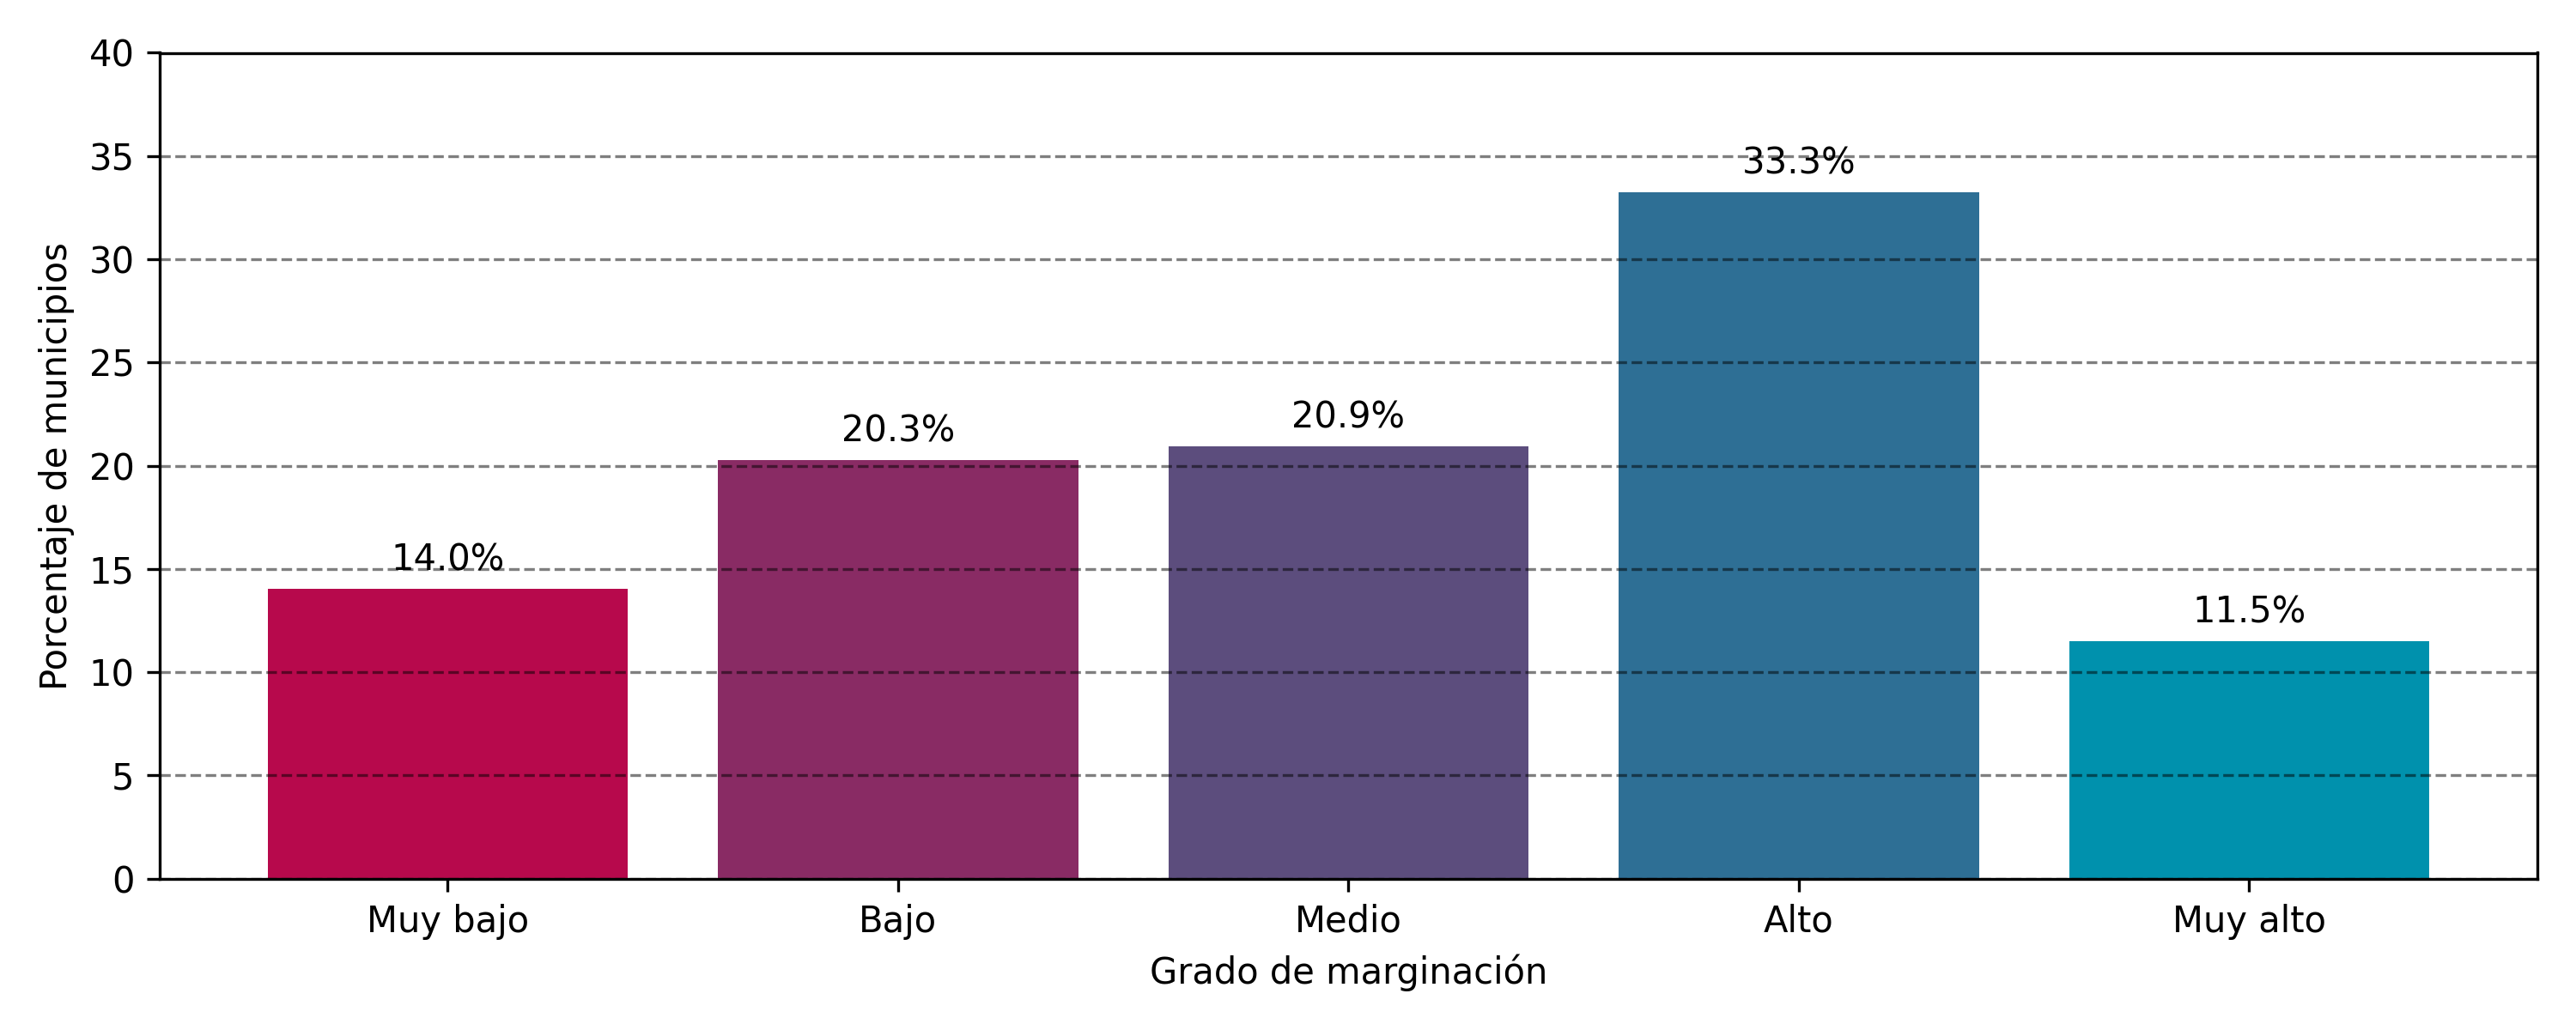
\includegraphics[width=1\linewidth]{Graphics/Data_2015/histogram_classes.png}
    \end{subfigure}
    \begin{subfigure}{8.4cm}
        \caption{Año 2020}
        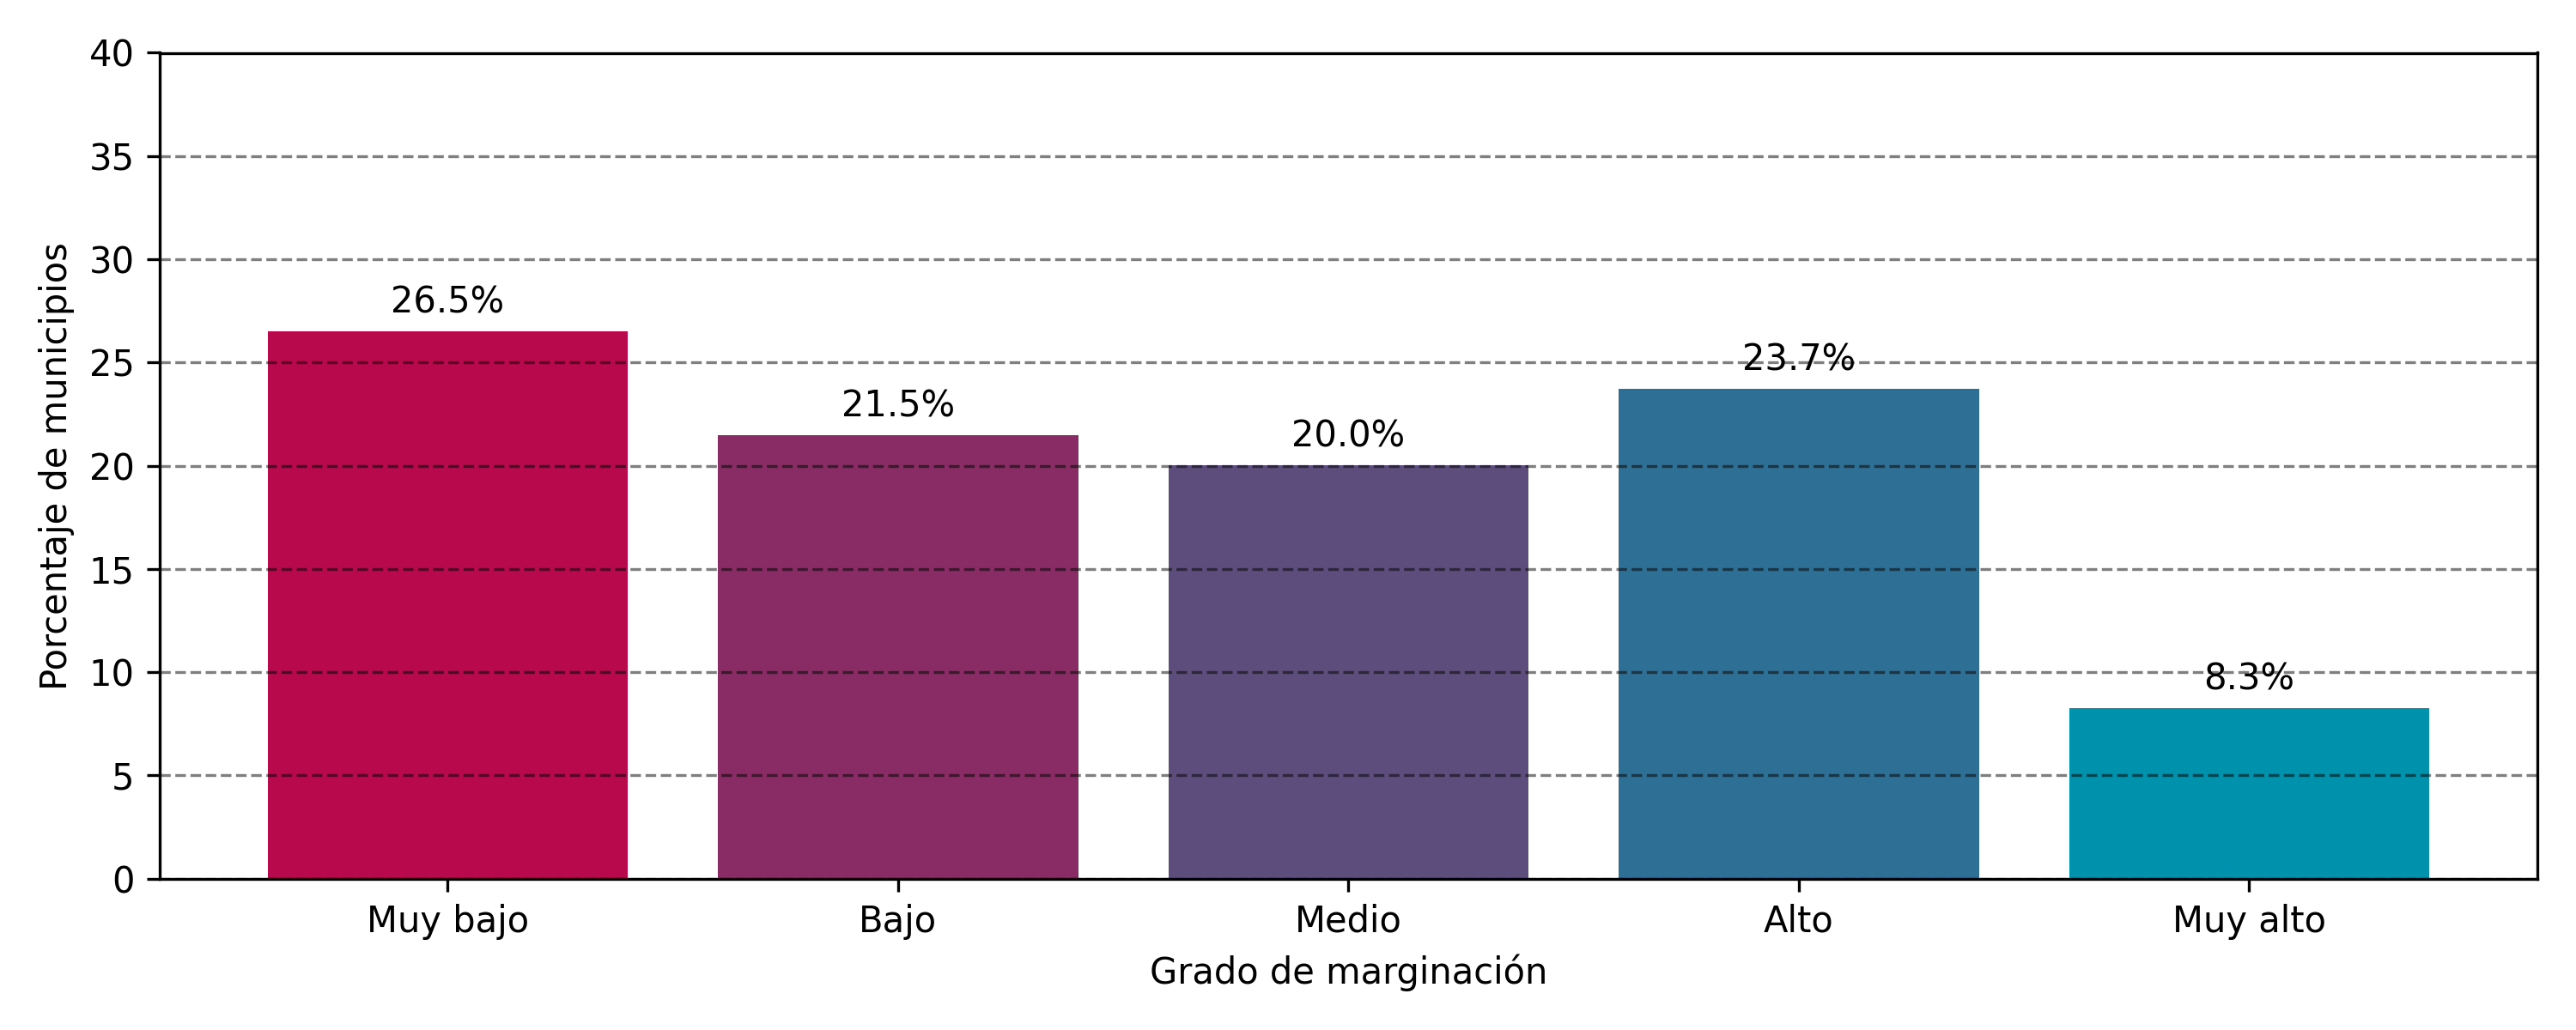
\includegraphics[width=1\linewidth]{Graphics/Data_2020/histogram_classes.png}
    \end{subfigure}
    \caption{Frecuencia relativa de cada índice de marginación en los años 2015-2020 a nivel municipio.}
    \label{fig:frecuency_relative}
\end{figure}

En la figura \ref{fig:map_mexico} se muestran los índices de marginacion para cada municipio en los años 2015 y 2020. Los datos para deliminar cada municipio fue obtenido del siguiente \href{https://blog.jjsantoso.com/mapas-distribucion-puntos/}{blog}\cite{mapa_mexico}.

\begin{figure}[H]
    \centering
    \begin{subfigure}{8.4cm}
        \caption{Año 2015}
        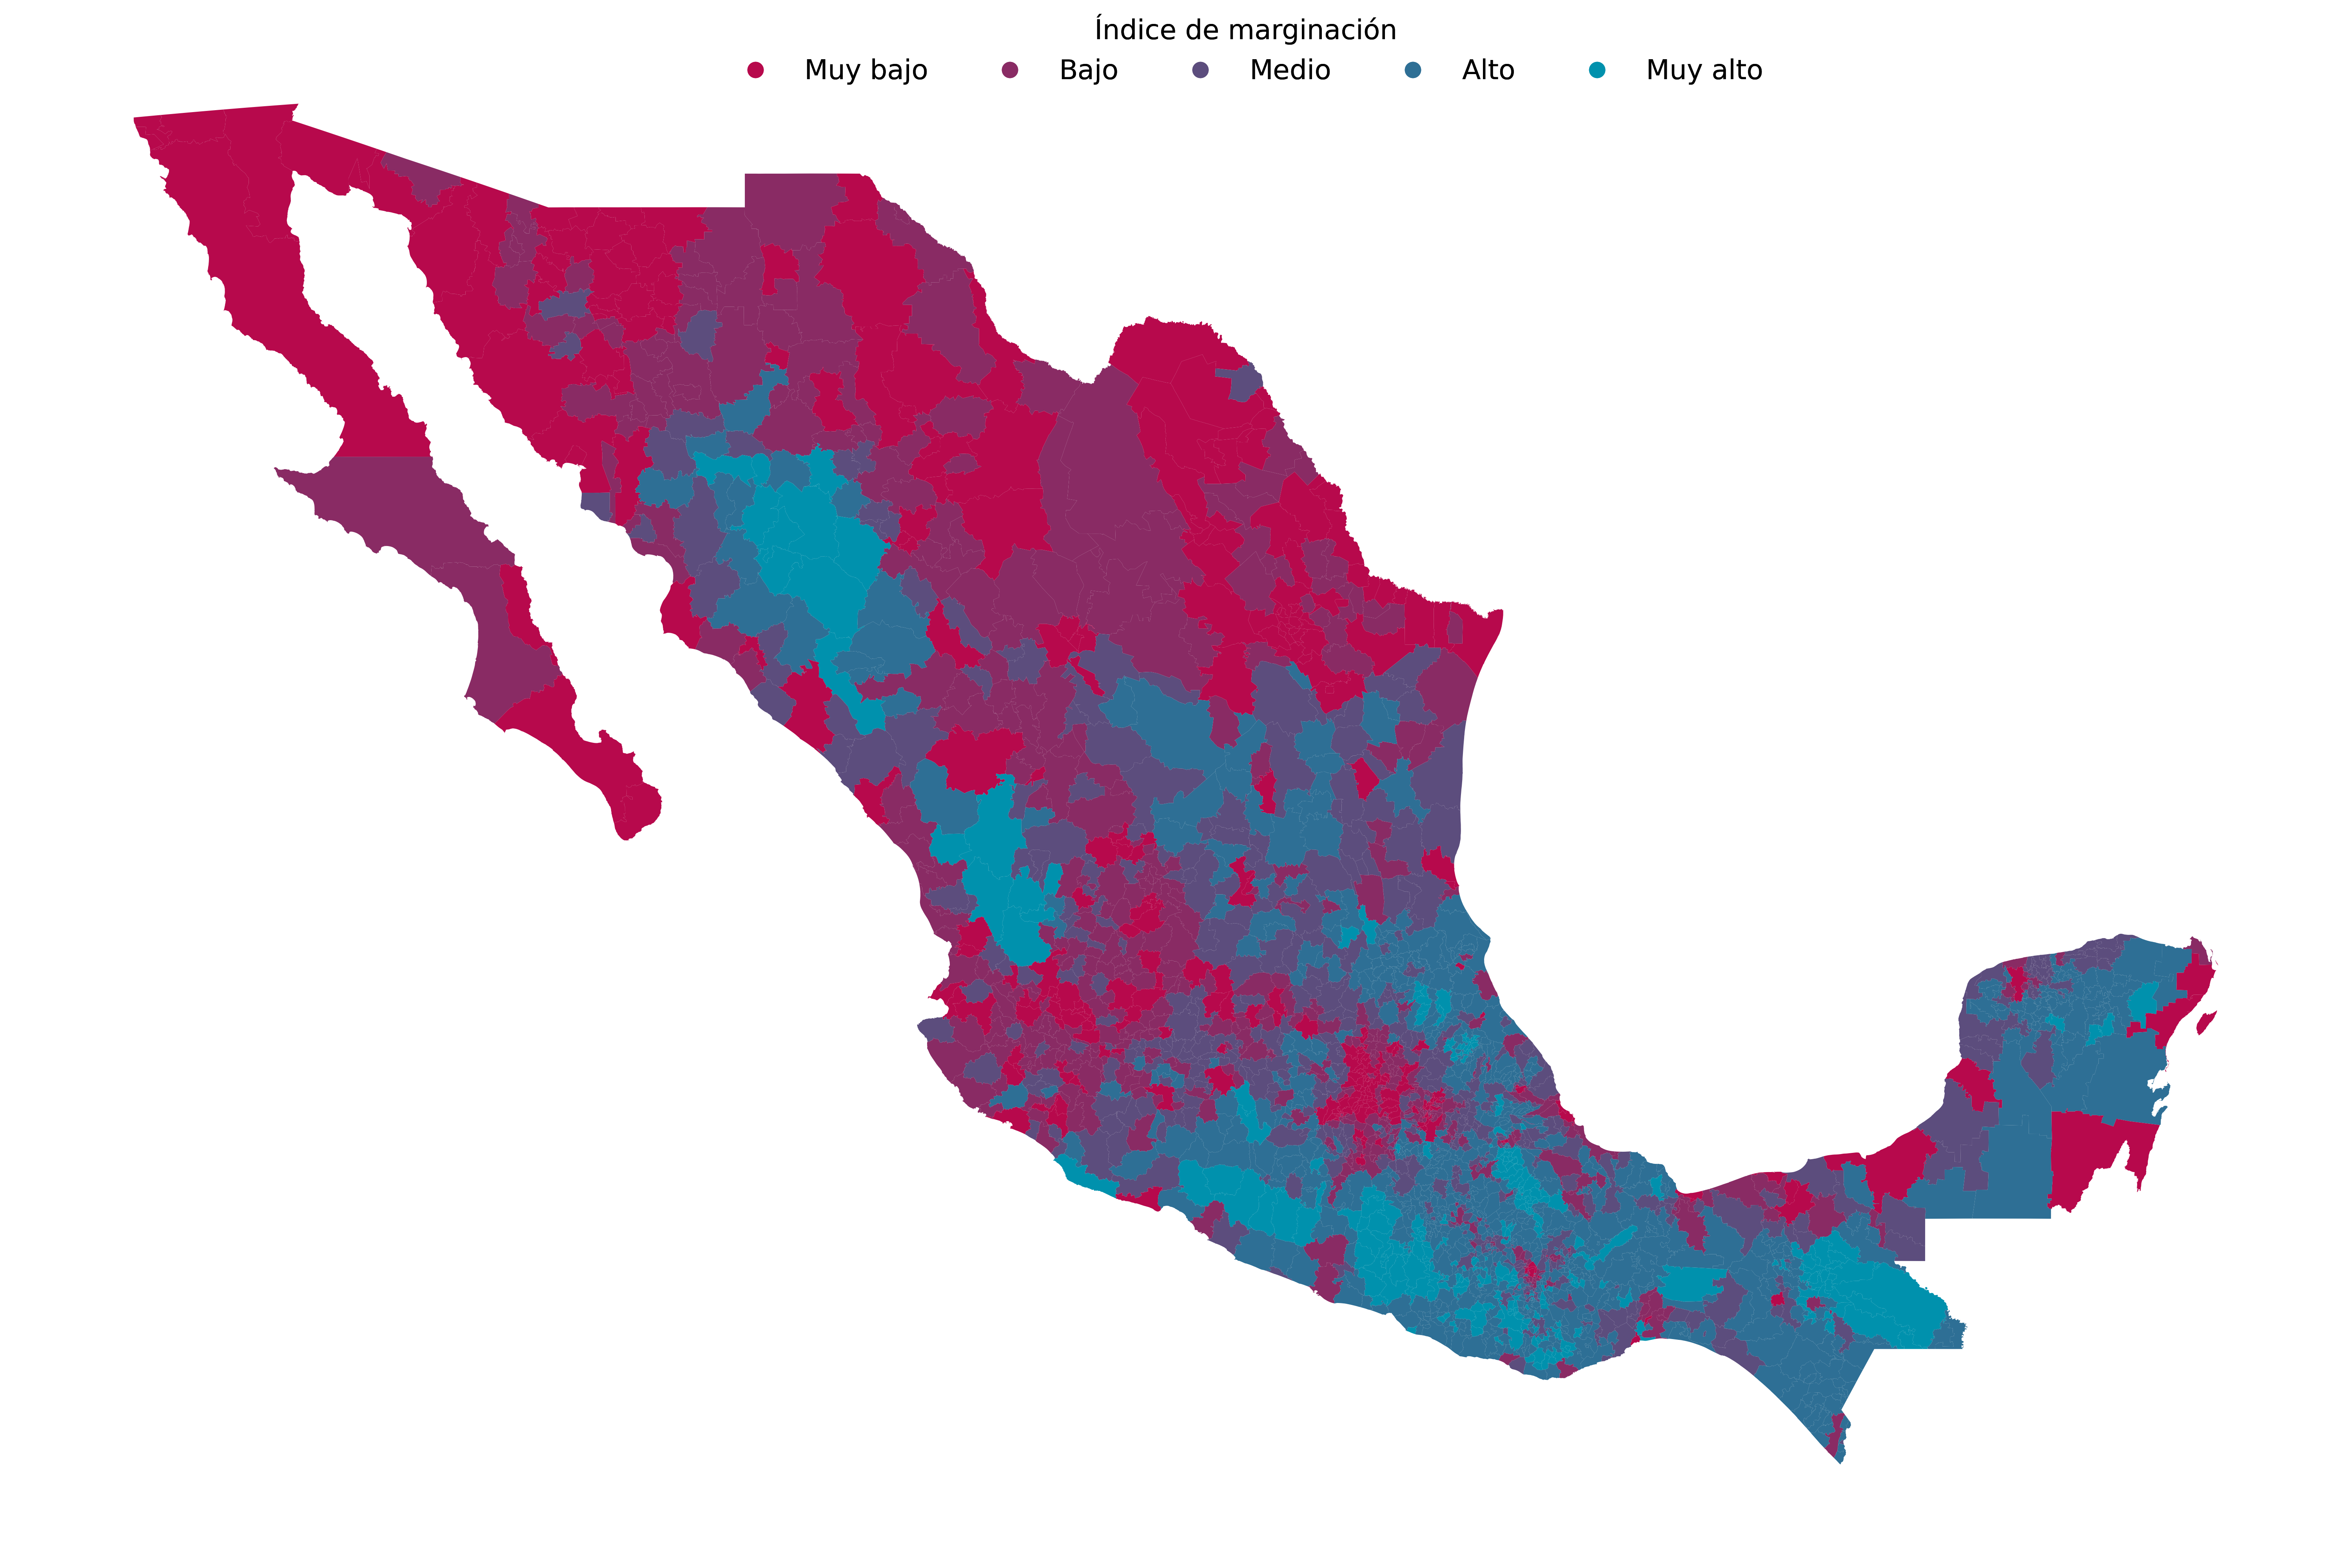
\includegraphics[width=1\linewidth]{Graphics/Data_2015/map.png}
    \end{subfigure}
    \begin{subfigure}{8.4cm}
        \caption{Año 2020}
        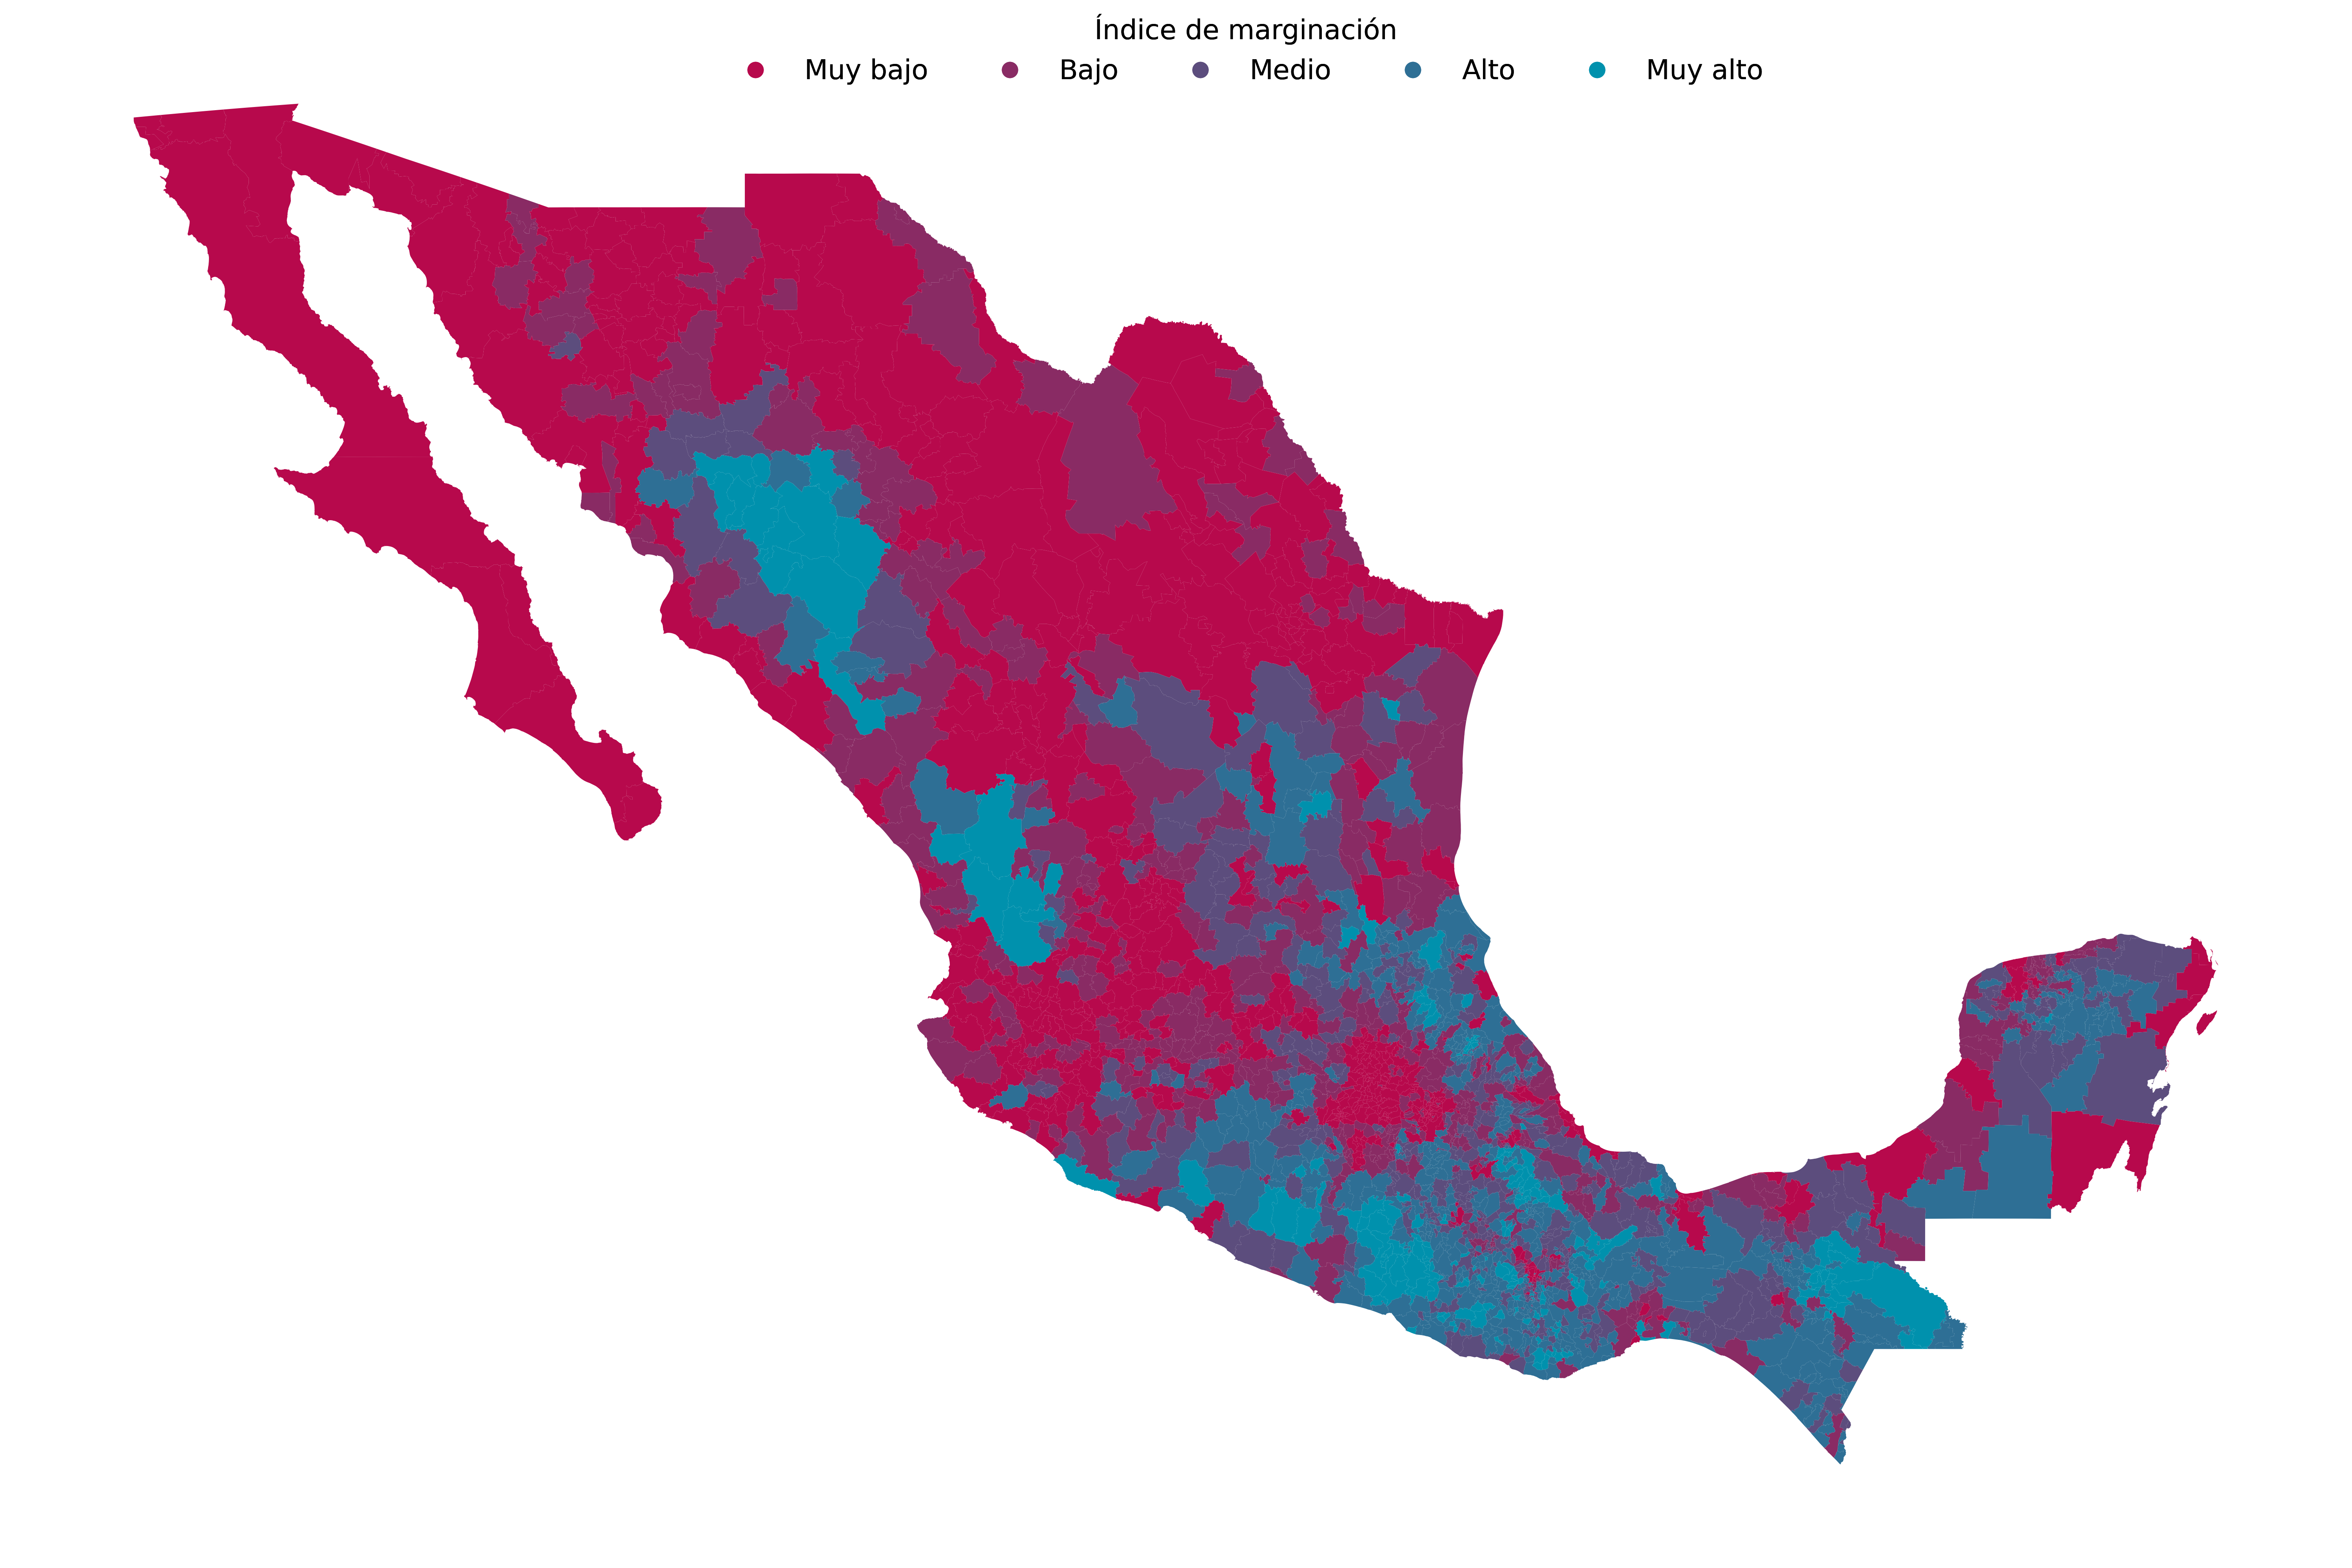
\includegraphics[width=1\linewidth]{Graphics/Data_2020/map.png}
    \end{subfigure}
    \caption{Grado de marginación a nivel municipio en la República Mexicana.}
    \label{fig:map_mexico}
\end{figure}